%%=============================================================================
%% Methodologie
%%=============================================================================

\chapter{Methodologie}
\label{ch:methodologie}

%% TODO: Hoe ben je te werk gegaan? Verdeel je onderzoek in grote fasen, en
%% licht in elke fase toe welke stappen je gevolgd hebt. Verantwoord waarom je
%% op deze manier te werk gegaan bent. Je moet kunnen aantonen dat je de best
%% mogelijke manier toegepast hebt om een antwoord te vinden op de
%% onderzoeksvraag.

\section{PWA Componenten}
Om een progressive web app te maken zijn er enkele belangrijke componenten. Deze gaan er voor zorgen dat je een optimale user experience krijgt net zoals je een native app zou hebben.
\begin{itemize}  
	\item Application shell
	\item Web App Manifest
	\item Service Worker
\end{itemize}

\subsection{Web App Manifest}
\lstset{
	string=[s]{"}{"},
	stringstyle=\color{blue},
	comment=[l]{:},
	commentstyle=\color{black},
}
Je web app manifest is een simpel JSON bestand waarin je aan de browser vertelt over je web app en hoe het zich moet gedragen als het geïnstalleerd wordt op het apparaat van de gebruiker. Zonder dit manifest zal Chrome nooit de optie geven aan de gebruiker om de app te installeren op het hoofdscherm (zie figuur \ref{fig:promptHome} ) \\

Een typisch manifest ziet er als volgt uit: 
	\begin{lstlisting}
{
"name": "Instagram als Progressive Web App",
"short_name": "PWAGram",
"icons": [
{
"src": "/src/images/icons/app-icon-48x48.png",
"type": "image/png",
"sizes": "48x48"
},
{
"src": "/src/images/icons/app-icon-96x96.png",
"type": "image/png",
"sizes": "96x96"
},
{
"src": "/src/images/icons/app-icon-144x144.png",
"type": "image/png",
"sizes": "144x144"
},
{
"src": "/src/images/icons/app-icon-192x192.png",
"type": "image/png",
"sizes": "192x192"
},
{
"src": "/src/images/icons/app-icon-256x256.png",
"type": "image/png",
"sizes": "256x256"
},
{
"src": "/src/images/icons/app-icon-384x384.png",
"type": "image/png",
"sizes": "384x384"
},
{
"src": "/src/images/icons/app-icon-512x512.png",
"type": "image/png",
"sizes": "512x512"
}
],
"start_url": "/index.html",
"scope": ".",
"display": "standalone",
"orientation": "portrait-primary",
"background_color": "#fff",
"theme_color": "#3f51b5",
"description": "Een simpele Instagram Clone.",
"dir": "ltr",
"lang": "nl-BE"
}
\end{lstlisting}


\clearpage
\begin{itemize}  
	\item name en short\_name: \\
	Eén van deze twee moet zeker aanwezig zijn. Als beide voorzien zijn zal overal de short\_name gebruikt worden waar de plaats beperkt is zoals op je hoofdscherm onder het icoon.
	\\
	\item icons \\
	Hier kun je je iconen definiëren. Je definiëert een lijst met je iconen. De browser zal dan de beste uitpakken voor hetgeen nodig is. Als de browser het icoon nodig heeft voor te tonen op je hoofdscherm zal hij hier hetgeen met de juiste afmetingen bepalen.
	\\
	\item start\_url: \\
	Dit vertelt aan de browser welke startpagina getoond moet worden aan de gebruiker. 
	\\
	\item scope: \\
	Welke pagina's zijn deel van de progressive web app en kunnen dus gebruik maken van de iconen en kleuren die zijn gedefiniëerd. Het is gebruikelijk om hier alle pagina's te kiezen. Dit kan door gewoon "." te zetten. 
	\\

	\item display: \\
	Hier kun je specifiëren welk deel van de browser getoond moet worden. Je kan aan de gebruiker nog steeds de adresbar tonen of je kan ervoor kiezen om alles te verbergen zodat het meer als een native app aanvoelt. \\
	\bigbreak
	\begin{longtable}
		\begin{tabular}{| p{.20\textwidth} | p{.80\textwidth} |}
			\hline
			\textbf{Waardes} & \textbf{Beschrijving} & & \\
			\hline
		
			 \textbf{fullscreen} & Neemt het geheel van plaats in beslag op het scherm en toont geen andere elementen. &  &  \\ 
			\hline
			\textbf{standalone} & De webapp zal eruit zien als een echte native app. Het opent op een apart venster, apart van de browser en toont geen standaard browser elementen zoals de zoekbalk. &  &  \\
			\hline
			\textbf{minimal-ui} & Dit wordt niet ondersteund in chrome. Hierbij heb je net hetzelfde als bij fullscreen maar je hebt een minimaal aantal aan elementen die je kan zien zoals een back-knop. &  &  \\
			\hline
			 \textbf{browser} & Het lijkt alsof je gewoon in de browser kijkt. &  & \\
			\hline
		\end{tabular}
	\end{longtable}

	\item background\_color: \\
De achtergrondkleur van de app. Dit wordt vooral getoond in laadschermen. Hiervoor gebruik je een hexadecimale code bv: #fff
\\


	\item theme\_color: \\
	Je thema kleur. Net zoals native apps een thema kleur hebben die gaat bepalen welke kleur je balk aan de top van je scherm heeft. Ook hier wordt gebruik gemaakt van een hexadecimale code
	\\
	\item description: \\
	Hier kan je een kleine samenvatting geven. Als een internetbrowser dit nodig heeft, zal hij dit hier vandaan halen. De gebruiker zal dit dus te zien krijgen.	
	\\
	\item dir \\
	Dit is de richting van je tekst. Doorgaans wordt hier ltr gebruikt, left to right. Als je wil kan je hier ook rtl kiezen.
	\\
	\item lang \\
	De taal van je app: je gebruikt hier de 4 letter code van de taal die je wil.
	\\
	\item orientation \\
	Hier kan je bepalen hoe je wil dat je app getoond wordt. Wil je dit rechtop of liever gedraaid. Je kan hier aan de gebruiker opleggen dat je het scherm niet kunt draaien. vb: portrait-primary
	\\
	
\end{itemize}


Na het toevoegen van je manifest moet je aan al je pagina's de link naar je manifest toevoegen.
\begin{lstlisting}
<link rel="manifest" href="/manifest.json">
\end{lstlisting}

Nadien kan je je manifest controleren in de developer tools van Google Chrome


	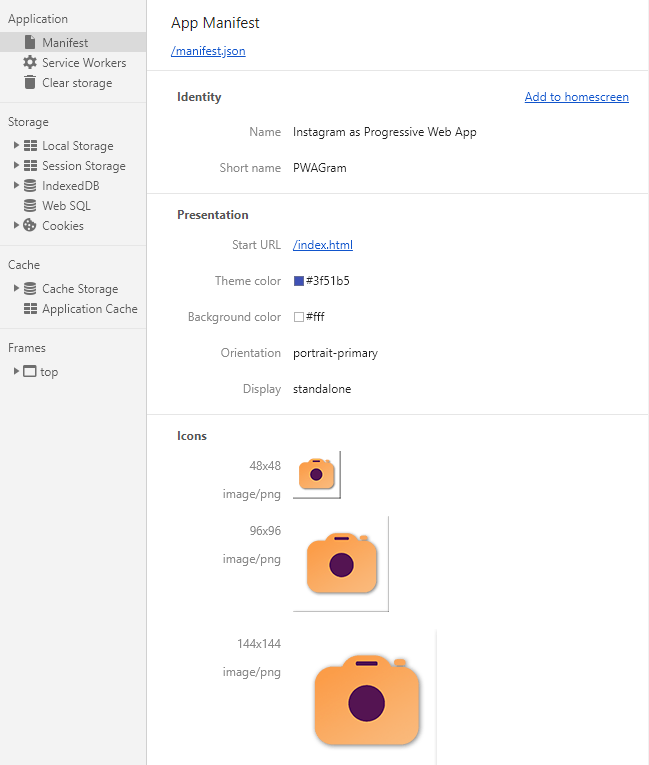
\includegraphics[scale=0.5]{img/manifestDev.png}



\subsection{Service Worker}
Het web is handig. Wil je de openingsuren van een winkel weten of wil je opzoeken wat ze allemaal verkopen? Ga naar hun website en je vindt het meteen. Het is zo makkelijk. En toch heeft iedereen al eens hetzelfde meegemaakt als ze dit willen doen: \\

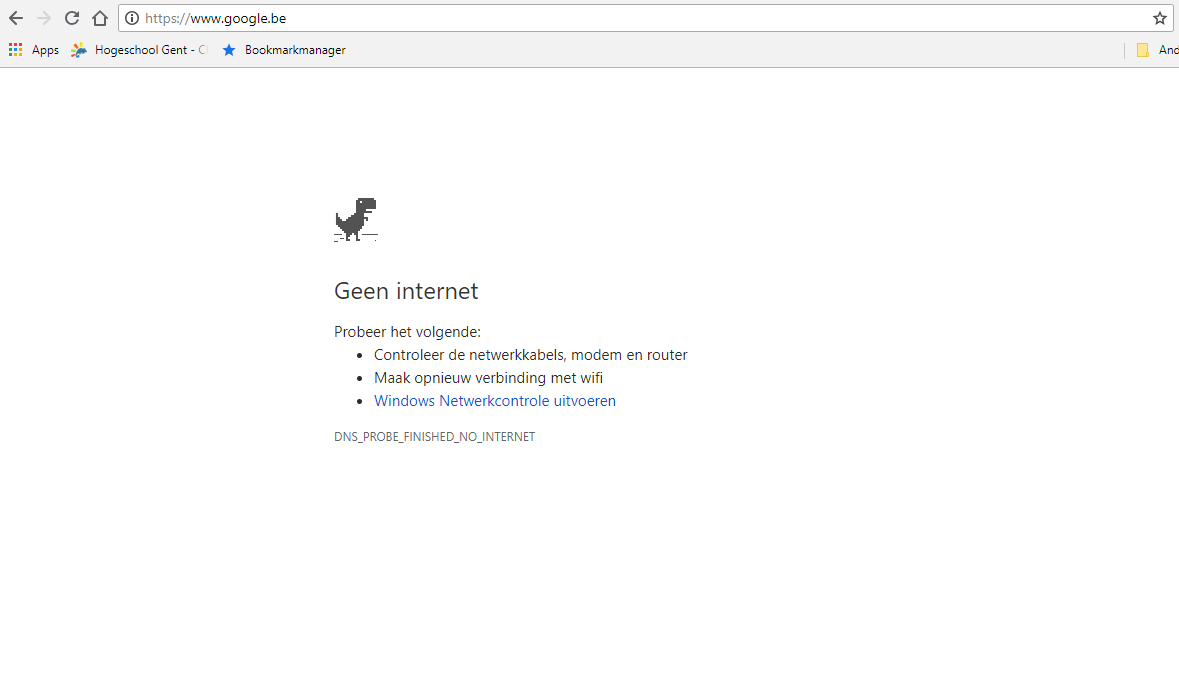
\includegraphics[scale=0.5]{img/noInternet.png}


Zoals je ziet kun je niet veel zien als je geen internet hebt. Zonder internet kan je niet de informatie gaan opzoeken die je nodig hebt.

Door de introductie van de service worker is dit voor ontwikkelaars niet langer een probleem en kunnen ze dit op een juiste manier verwerken zodat de gebruikers niet merken dat ze geen internet hebben. Dit is de belangrijkste taak van de service worker maar lang niet de enige.

Een service worker is een script dat, apart van de webpagina, op de browser draait. Hierdoor zijn er verschillende functionaliteiten die gebruikt kunnen worden waarbij geen interactie van de gebruiker nodig is. Momenteel zijn dit functionaliteiten zoals push notificaties of offline gebruik van de site maar wie weet welke functionaliteiten in de toekomst nog mogelijk zullen worden gemaakt. 


Aangezien een service worker apart loopt van de webpagina heeft het ook een andere levenscyclus. 

	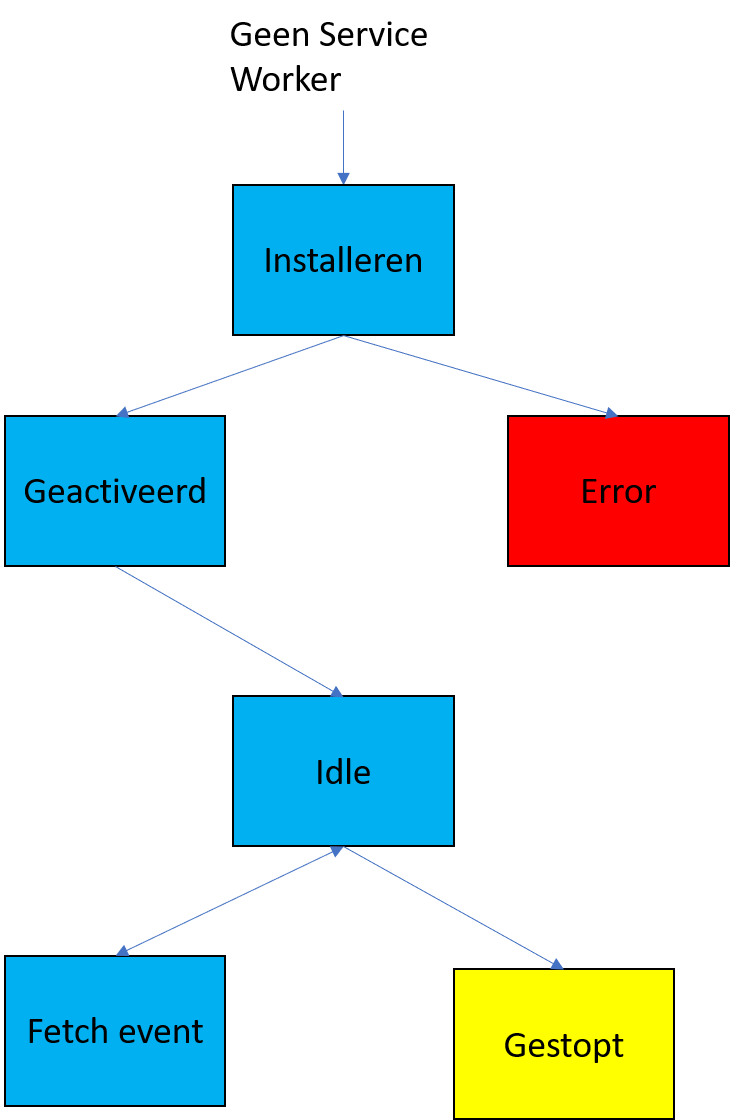
\includegraphics[scale=0.5]{img/lifeCycle.png}
	
	Voordat de service worker kan geïnstalleerd worden moeten we deze eerst registreren.
	
\begin{lstlisting}
if ('serviceWorker' in navigator) {
window.addEventListener('load', function() {
navigator.serviceWorker.register('/sw.js').then(function(registration) {
// Registration was successful
console.log('ServiceWorker registration successful with scope: ', registration.scope);
}, function(err) {
// registration failed :(
console.log('ServiceWorker registration failed: ', err);
});
});
}
\end{lstlisting}

Als je je service worker geregistreerd hebt, zal de browser deze direct installeren op de achtergrond. Je kan vanaf nu ook je service worker bekijken in de developer tools van Chrome (zie figuur \ref{fig:swDev}).

Tijdens het installeren kan je in het script meegeven wat het moet doen. In de meeste gevallen zal hier ook het cachen van statiche bestanden gebeuren. Aangezien deze statisch zijn en weinig veranderingen nodig hebben hoeft dit eenmalig te gebeuren, tijdens de installatie. Als bestanden niet kunnen gecached worden dan zal de installatiestap falen en zal deze nooit geactiveerd worden. De volgende keer zal de browser opnieuw proberen de service worker te installeren.
\begin{lstlisting}
var CACHE_NAME = 'my-site-cache-v1';
var urlsToCache = [
'/',
'/styles/main.css',
'/script/main.js'
];

self.addEventListener('install', function(event) {
// Perform install steps
event.waitUntil(
caches.open(CACHE_NAME)
.then(function(cache) {
console.log('Opened cache');
return cache.addAll(urlsToCache);
})
);
});
\end{lstlisting}


Nadat de service worker geïnstalleerd is wordt deze geactiveerd. Dit is de ideale plaats om oude caches te verwijderen en te zorgen dat de data die wel bewaard wordt up to date is.

Wanneer een service worker geactiveerd is wacht deze. Dit noemen we idle-state. De service worker wacht tot hij een taak toegewezen krijgt. Dit gebeurt als er een fetch-evenement wordt opgeroepen. In dit geval komt de service worker tot leven en zal hij deze taak uitvoeren waarna hij weer in een idle-state beland. De service worker zal in deze staat blijven tot deze wordt geüpdate. Hierdoor kan deze reageren op events zoals push-notificaties, zelfs als de web app gesloten is.

Je kan als ontwikkelaar zelf events toevoegen waarop de service worker zal reageren zoals het aanklikken van een notificatie

\begin{lstlisting}
self.addEventListener('notificationclick', function (event) {
var action = event.action;

console.log(notification);

if (action === 'confirm') {
console.log('Confirm was chosen');
} else {
console.log('Another action was chosen');
}
});
\end{lstlisting}

Maar het belangrijkste event is het fetch event. Deze zal de dynamische inhoud van je webpagina laden. Door het juist implementeren van dit event kan je ervoor zorgen dat de gebruiker het niet merkt als hij geen internetverbinding zou hebben.


\clearpage
\subsubsection{Offline gebruik}
\begin{lstlisting}
self.addEventListener('fetch', function (event) {
console.log('Haal de dynamische data op.');
});
\end{lstlisting}

Het offline gebruiken van een progressive web app is één van de belangrijkste eigenschappen. Gebruikers zonder internetverbinding kunnen nog steeds je web app blijven gebruiken. Dit geldt ook voor gebruikers met een slechte verbinding. Ondanks hun verbinding zullen ze geen wachttijden te zien krijgen. Dit is als bedrijf heel goed aangezien gebruikers sneller zullen afhaken als ze moeten wachten tot een pagina geladen is.

Voor het ophalen van data zijn er enkele manieren waarop je te werk kan gaan. Afhankelijk van wat je wil zul je het fetch-event anders implementeren.
 
\begin{itemize}
	\item Netwerk-only: Bij een fetch event zal de service worker de gegevens enkel ophalen over het netwerk. Hierdoor zal de gebruiker altijd de laatste gegevens hebben. Het offline gebruiken van de app zal niet mogelijk zijn aangezien het gegevens steeds over het internet wil ophalen.
	\item Cache-only: De gebruiker zal de gegevens altijd van de cache ophalen. Gegevens die op het netwerk worden aangepast zullen hier niet zichtbaar zijn aangezien ze nooit worden opgehaald. Dit is ideaal voor statische gegevens die nooit worden aangepast. Doordat het over de cache gaat en niet over het netwerk gaat dit veel sneller.
	\item Cache dan netwerk: De data wordt eerst opgehaald uit de cache en nadien via het netwerk. Eenmaal de gegevens van het netwerk zijn opgehaald wordt de pagina aangepast met de nieuwste data. Dit is ideaal waar data altijd up-to-date moet zijn zoals scoreborden en nieuwsartikelen.
	\item Cache met netwerk alternatief: De service worker zal de gegevens die hij daar terugvind ophalen uit de cache en alles waarvan hij een nieuwere versie vind op het netwerk van daar. Je zal hierdoor altijd de nieuwste versie hebben. Tijdens dit kan je ook je cache updaten waardoor de gebruiker de laatste versie in zijn cache heeft en de volgende keer hij die pagina bezoekt er minder moet worden opgehaald over het netwerk. 
	\item Netwerk met cache alternatief: De service worker haalt de gegevens op via het netwerk. Hierdoor krijgt de gebruiker altijd de laatste gegevens te zien. Als de service worker hierbij problemen ondervind door een slechte verbinding zal hij de gegevens uit de cache ophalen. Hierdoor kan een gebruiker met een slechte verbinding lang moeten wachten voor hij data ziet.
\end{itemize}

\subsection{Application shell}
De application of app shell is het minimum aan HTML, CSS en Javascript dat je nodig hebt om je applicatie te kunnen tonen. Dit minimum wordt gecached zodat dit zelfs zonder internetverbinding altijd snel getoond kan worden aan de gebruiker. Hierdoor hoeft enkel de dynamische inhoud zoals een artikel geladen te worden via het netwerk.
De app shell is heel handig om al iets te kunnen tonen aan de gebruiker terwijl andere delen nog tijd nodig hebben om te laden.
\begin{figure}[h]
	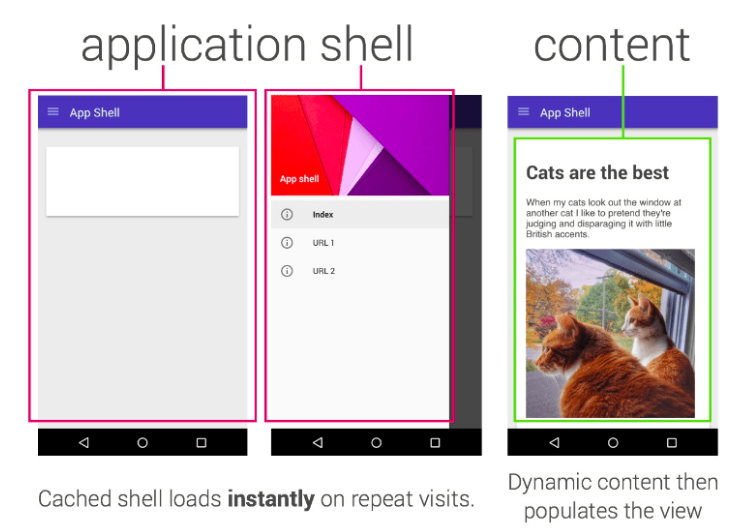
\includegraphics[scale=0.5]{img/appShell.png}
	\caption{Application shell}
	\label{fig:appShell}
\end{figure}
Zoals je op afbeelding \ref{fig:appShell} ziet, heb je in de application shell het minimum dat je wil tonen aan de gebruiker. Wanneer je de app ook bezoekt, zal dit altijd hetzelfde zijn. Aangezien hier weinig of geen verandering is, kan je dit lokaal opslaan (cachen). Het dynamisch gedeelte, het artikel, wordt wel via het netwerk geladen. Dit gedeelte, de inhoud, is niet altijd hetzelfde en zal vaak veranderen. Het is dus niet nodig dit lokaal op te slaan. Als er toch updates aan bestanden van de app shell worden gedaan, zal de progressive web app dit zien. De volgende keer dat de gebruiker online is, zal de app de oude bestanden vervangen door de nieuwe. Als ontwikkelaar is het belangrijk op voorhand te kijken welke bestanden je gaat cachen en welke niet.
Belangrijke voorwaarden voor de app shell zijn: 
\begin{itemize}  
	\item Snel laden
	\item Zo weinig mogelijk data gebruiken
	\item Statische bestanden gebruiken van de lokale cache
	\item Inhoud en navigatie scheiden
\end{itemize}

Dit is een voorbeeld van een app shell waarbij het sw.js bestand wordt gecachet. 
\lstdefinelanguage{JavaScript}{
	morekeywords={typeof, new, true, false, catch, function, return, null, catch, switch, var, if, in, while, do, else, case, break},
	morecomment=[s]{/*}{*/},
	morecomment=[l]//,
	morestring=[b]",
	morestring=[b]'
}
\lstdefinelanguage{HTML5}{
	language=html,
	sensitive=true, 
	alsoletter={<>=-},
	otherkeywords={
		% HTML tags
		<html>, <head>, <title>, </title>, <meta, />, </head>, <body>,
		<canvas, \/canvas>, <script>, </script>, </body>, </html>, <!, html>, <style>, </style>, ><
	},  
	ndkeywords={
		% General
		=,
		% HTML attributes
		charset=, id=, width=, height=,
		% CSS properties
		border:, transform:, -moz-transform:, transition-duration:, transition-property:, transition-timing-function:
	},  
	morecomment=[s]{<!--}{-->},
	tag=[s]
}


\begin{lstlisting}
<!DOCTYPE html>
<html>
<head>
<meta charset="utf-8">
<title>App Shell</title>
<link rel="manifest" href="/manifest.json">
<meta http-equiv="X-UA-Compatible" content="IE=edge">
<meta name="viewport" content="width=device-width, initial-scale=1.0">
<link rel="stylesheet" type="text/css" href="styles/inline.css">
</head>

<body>
<header class="header">
<h1 class="header__title">App Shell</h1>
</header>

<nav class="nav"></nav>

<main class="main"></main>

<div class="dialog-container"></div>

<div class="loader">
<!-- Show a spinner or placeholders for content -->
</div>

<script src="app.js" async></script>
<script>
if ('serviceWorker' in navigator) {
navigator.serviceWorker.register('/sw.js').then(function(registration) {
// Registration was successful
console.log('ServiceWorker registration successful with scope: ', registration.scope);
}).catch(function(err) {
// registration failed :(
console.log('ServiceWorker registration failed: ', err);
});
}
</script>
</body>
</html>
\end{lstlisting}

\subsection{Lighthouse}
Na het creëren van je progressive web app, kan je deze laten auditeren door lighthouse. Je progressive web app krijgt een rapport speciaal voor jou opgemaakt. Je krijgt hier een score (op 100) op verschillende punten). Het rapport toont ook waar je nog dingen kunt verbeteren.


	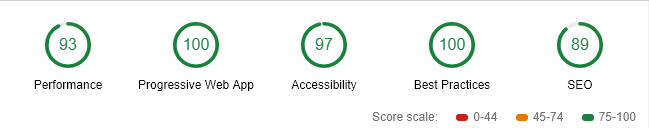
\includegraphics[scale=1]{img/audit.png}


\begin{itemize}  
	\item Performance: Dit toont hoe goed je huidige app presteert. Dit zal onder andere meten hoe snel de pagina laad.
	\item Progressive web app: In welke mate voldoet de app aan de checklist waaraan een progressive web app moet voldoen. Dit gaat ondere andere kijken of er een pictogram is voor het hoofdscherm van een telefoon.
	\item Accessibility: Hoe toegankelijk is je app. Hier kan je een goede score krijgen door onder andere een goed kleurencontrast te gebruiken op je webpagina's.
	\item Best practices: Hou je je aan de best practices omtrent het schrijven van een web app. Hier wordt er onder andere gekeken of je geen error logs in de consoles toont.
	\item SEO: Is je pagina optimaal voor zoekmachines?
\end{itemize}


\section{PWA vs Native}
Met de komst van de progressive web app wordt de kloof tussen het web en native gedicht. Functionaliteiten van het apparaat die vroeger enkel door native apps konden gebruikt worden, zijn nu ook beschikbaar voor web apps. 

	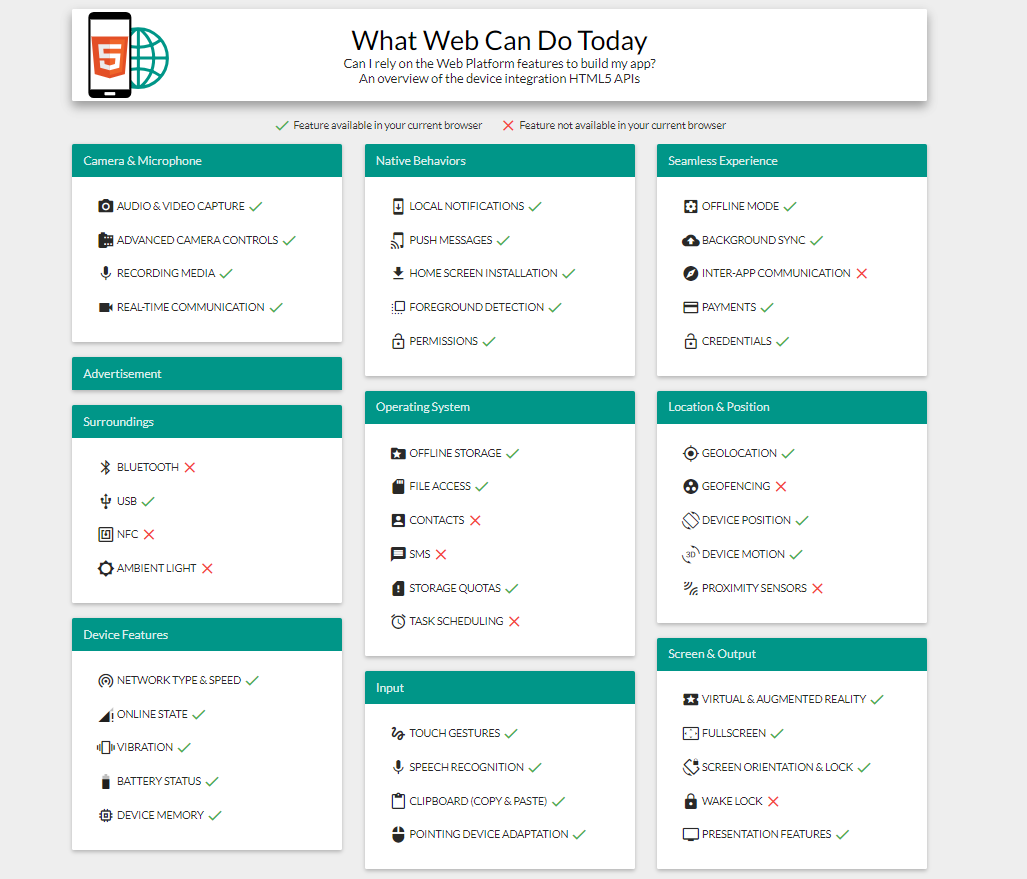
\includegraphics[scale=0.6]{img/webToday.png}
	
	\clearpage
	Ondanks dat native en web dichter naar mekaar groeien zijn er nog steeds enkele verschillen tussen beiden. Zo hebben ze elk enkele voordelen tegenover de ander.

\subsection{Voordelen native tegenover web}	
\begin{itemize}  
	\item Ondanks de vele functionaliteiten van het apparaat dat het web kan gebruiken zijn er toch nog enkele die enkel voor native voorbestemd zijn. Voor ontwikkelaars dat gebruik willen maken van deze specifieke functionaliteiten zullen voor een native app moeten kiezen
	\item App stores zijn niet altijd slecht. Gebruikers kunnen makkelijk nieuwe apps ontdekken. Ze kunnen er redelijk zeker van zijn dat de app die ze willen downloaden geen slechte bedoelingen heeft aangezien deze eerst gecontroleerd worden voor ze op de store geplaats kunnen worden. Als bedrijf kun je beoordelingen krijgen die je kan gebruiken om je app te verbeteren.
	\item Wake lock zorgt ervoor dat je scherm niet uitgaat na een bepaalde tijd van inactiviteit. Als je de Netflix-app gebruikt wil je niet elke vijf minuten je scherm aanraken zodat het niet uitvalt. Web apps kunnen deze wake lock niet gebruiken waardoor het zomaar kan gebeuren dat, in het midden van je artikel dat je aan het lezen bent, je telefoon uitvalt.
\end{itemize}

\subsection{Voordelen web tegenover native}	
	
\begin{itemize}  
	\item Inhoud in progressive web apps kan makkelijk gevonden worden door zoekmachines. Voor native apps wordt er niet gekeken naar inhoud. Native apps zoals Reddit zul je enkel terugvinden als je zoekt naar Reddit, maar niet als je zoekt naar één van de vele subreddits die Reddit rijk is. 
	\item Wil je een artikel delen die je hebt gezien in een online winkel? Bij een web app kan je makkelijke elke pagina linken en deze delen met anderen. Gebruikers hebben maar één link nodig om direct op een bepaalde pagina te komen. Bij native app moeten ze eerst via de app store om daar de app te downloaden. Nadien moeten ze nog navigeren naar de juiste pagina. 
	\item Als ontwikkelaar moet je niet elke update laten goedkeuren door de app store maar kan je je web app updaten wanneer je wil.
	\item Vanaf dat je web app online is, is het bereikbaar voor iedereen. Voordat je een native app kunt gebruiken moet je enkele stappen doorlopen. Bij elk van deze stappen verlies je ongeveer 20\% gebruikers. Als je bij 1000 mensen interesse hebt opgewekt voor je app, heb na alle stappen te doorlopen nog ongeveer 262 gebruikers over. (zie figuur \ref{fig:appDropOff})
\end{itemize}

